\documentclass[aspectratio=169]{../latex_main/tntbeamer}  % you can pass all options of the beamer class, e.g., 'handout' or 'aspectratio=43'
\usepackage{dsfont}
\usepackage{bm}
\usepackage[english]{babel}
\usepackage[T1]{fontenc}
%\usepackage[utf8]{inputenc}
\usepackage{graphicx}
\graphicspath{ {./figures/} }
\usepackage{algorithm}
\usepackage[ruled,vlined,algo2e,linesnumbered]{algorithm2e}
\usepackage{hyperref}
\usepackage{booktabs}
\usepackage{mathtools}

\usepackage{amsmath,amssymb}

\DeclareMathOperator*{\argmax}{arg\,max}
\DeclareMathOperator*{\argmin}{arg\,min}

\usepackage{amsbsy}
\newcommand{\vect}[1]{\bm{#1}}
%\newcommand{\vect}[1]{\boldsymbol{#1}}

\usepackage{pgfplots}
\pgfplotsset{compat=1.16}
\usepackage{tikz}
\usetikzlibrary{trees} 
\usetikzlibrary{shapes.geometric}
\usetikzlibrary{positioning,shapes,shadows,arrows,calc,mindmap}
\usetikzlibrary{positioning,fadings,through}
\usetikzlibrary{decorations.pathreplacing}
\usetikzlibrary{intersections}
\pgfdeclarelayer{background}
\pgfdeclarelayer{foreground}
\pgfsetlayers{background,main,foreground}
\tikzstyle{activity}=[rectangle, draw=black, rounded corners, text centered, text width=8em]
\tikzstyle{data}=[rectangle, draw=black, text centered, text width=8em]
\tikzstyle{myarrow}=[->, thick, draw=black]

% Define the layers to draw the diagram
\pgfdeclarelayer{background}
\pgfdeclarelayer{foreground}
\pgfsetlayers{background,main,foreground}

% Requires XeLaTeX or LuaLaTeX
%\usepackage{unicode-math}

\usepackage{fontspec}
%\setsansfont{Arial}
\setsansfont{RotisSansSerifStd}[ 
Path=../latex_main/fonts/,
Extension = .otf,
UprightFont = *-Regular,  % or *-Light
BoldFont = *-ExtraBold,  % or *-Bold
ItalicFont = *-Italic
]
\setmonofont{Cascadia Mono}[
Scale=0.8
]

\renewcommand{\ttdefault}{Cascadia Mono}

% scale factor adapted; mathrm font added (Benjamin Spitschan @TNT, 2021-06-01)
%\setmathfont[Scale=1.05]{Libertinus Math}
%\setmathrm[Scale=1.05]{Libertinus Math}

% other available math fonts are (not exhaustive)
% Latin Modern Math
% XITS Math
% Libertinus Math
% Asana Math
% Fira Math
% TeX Gyre Pagella Math
% TeX Gyre Bonum Math
% TeX Gyre Schola Math
% TeX Gyre Termes Math

% Literature References
\newcommand{\lit}[2]{\href{#2}{\footnotesize\color{black!60}[#1]}}

%%% Beamer Customization
%----------------------------------------------------------------------
% (Don't) Show sections in frame header. Options: 'sections', 'sections light', empty
\setbeamertemplate{headline}{empty}

% Add header logo for normal frames
\setheaderimage{
	% 
\includegraphics[height=\logoheight]{figures/TNT_darkv4.pdf}
	
\includegraphics[height=\logoheight]{../latex_main/figures/Leibniz-AI-Academy_Logo}
	% 
\includegraphics[height=\logoheight]{figures/logo_tntluh.pdf}
}

% Header logo for title page
\settitleheaderimage{
	% 
\includegraphics[height=\logoheight]{figures/TNT_darkv4.pdf}
	
\includegraphics[height=\logoheight]{../latex_main/figures/Leibniz-AI-Academy_Logo}
	% 
\includegraphics[height=\logoheight]{figures/logo_tntluh.pdf}
}

% Title page: tntdefault 
\setbeamertemplate{title page}[tntdefault]  % or luhstyle
% Add optional title image here
%\addtitlepageimagedefault{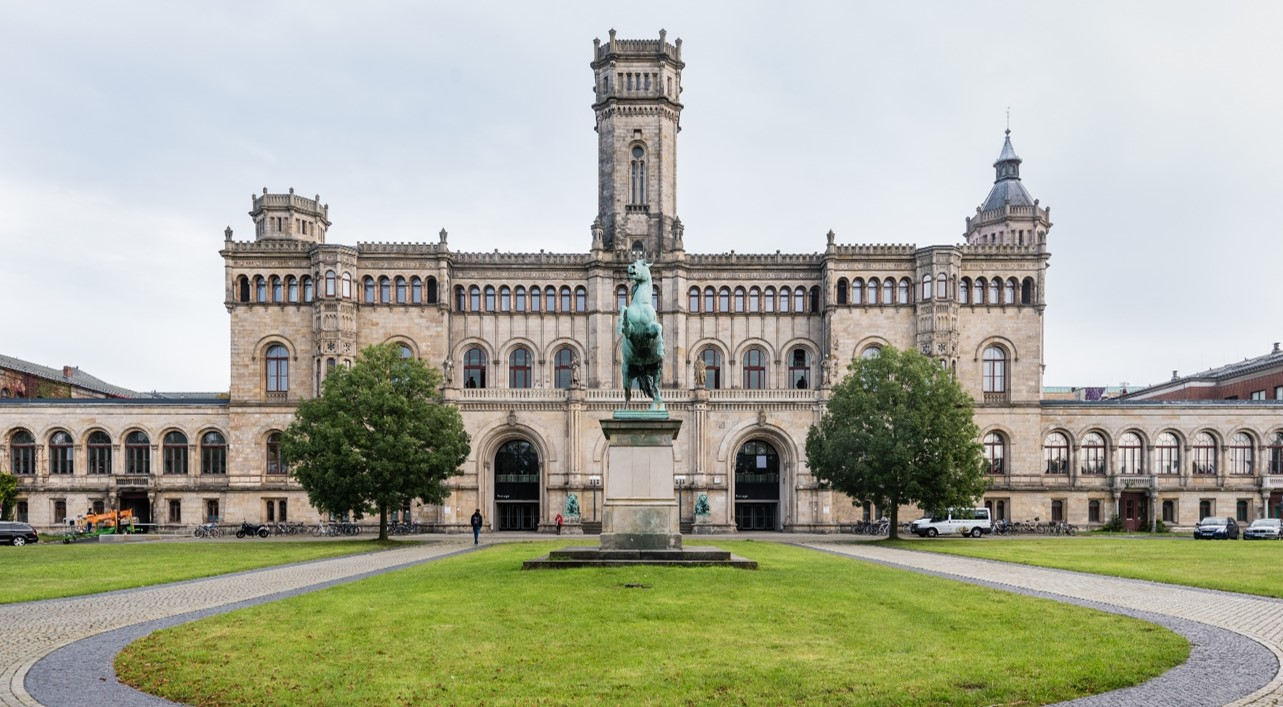
\includegraphics[width=0.65\textwidth]{figures/luh_default_presentation_title_image.jpg}}

% Title page: luhstyle
% \setbeamertemplate{title page}[luhstyle]
% % Add optional title image here
% \addtitlepageimage{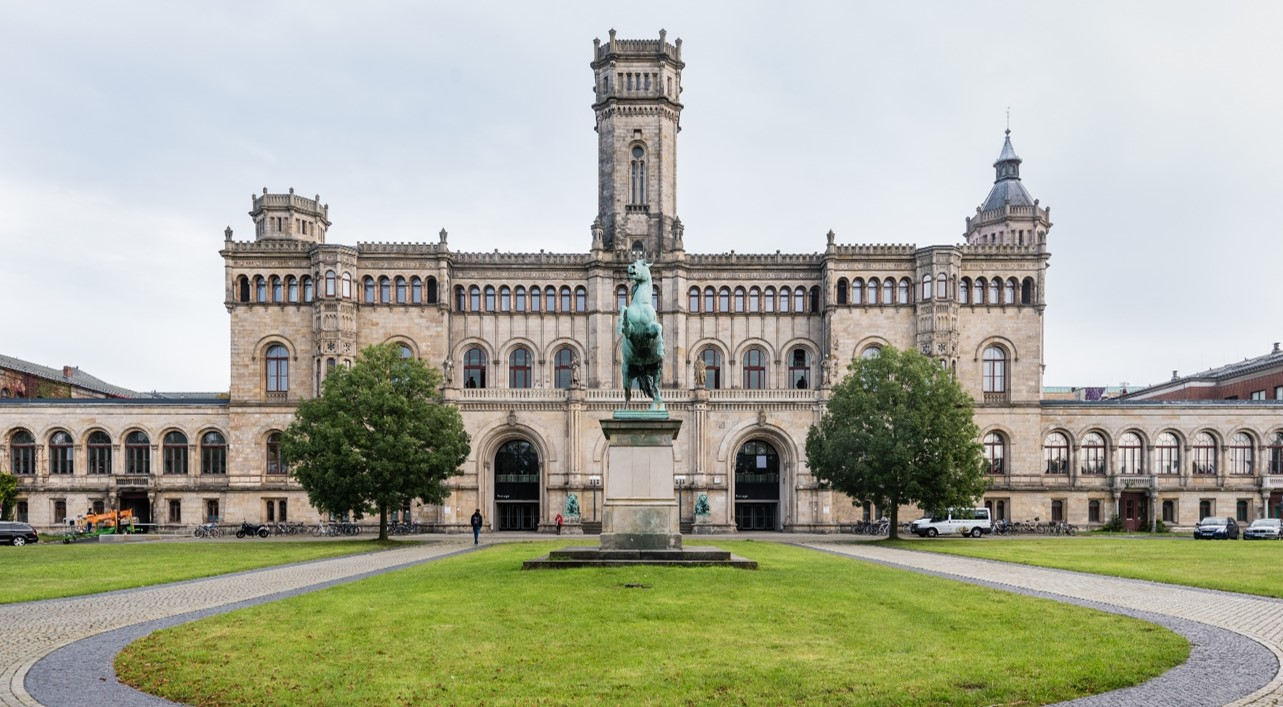
\includegraphics[width=0.75\textwidth]{figures/luh_default_presentation_title_image.jpg}}

\author[Abedjan \& Lindauer]{Ziawasch Abedjan \& \underline{Marius Lindauer}\\[1em]
	%
\includegraphics[height=\logoheight]{../latex_main/figures/luh_logo_rgb_0_80_155.pdf}\qquad
	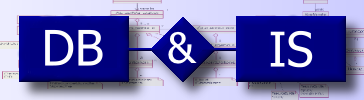
\includegraphics[height=\logoheight]{../latex_main/figures/DBIS_Kurzlogo.png}\qquad
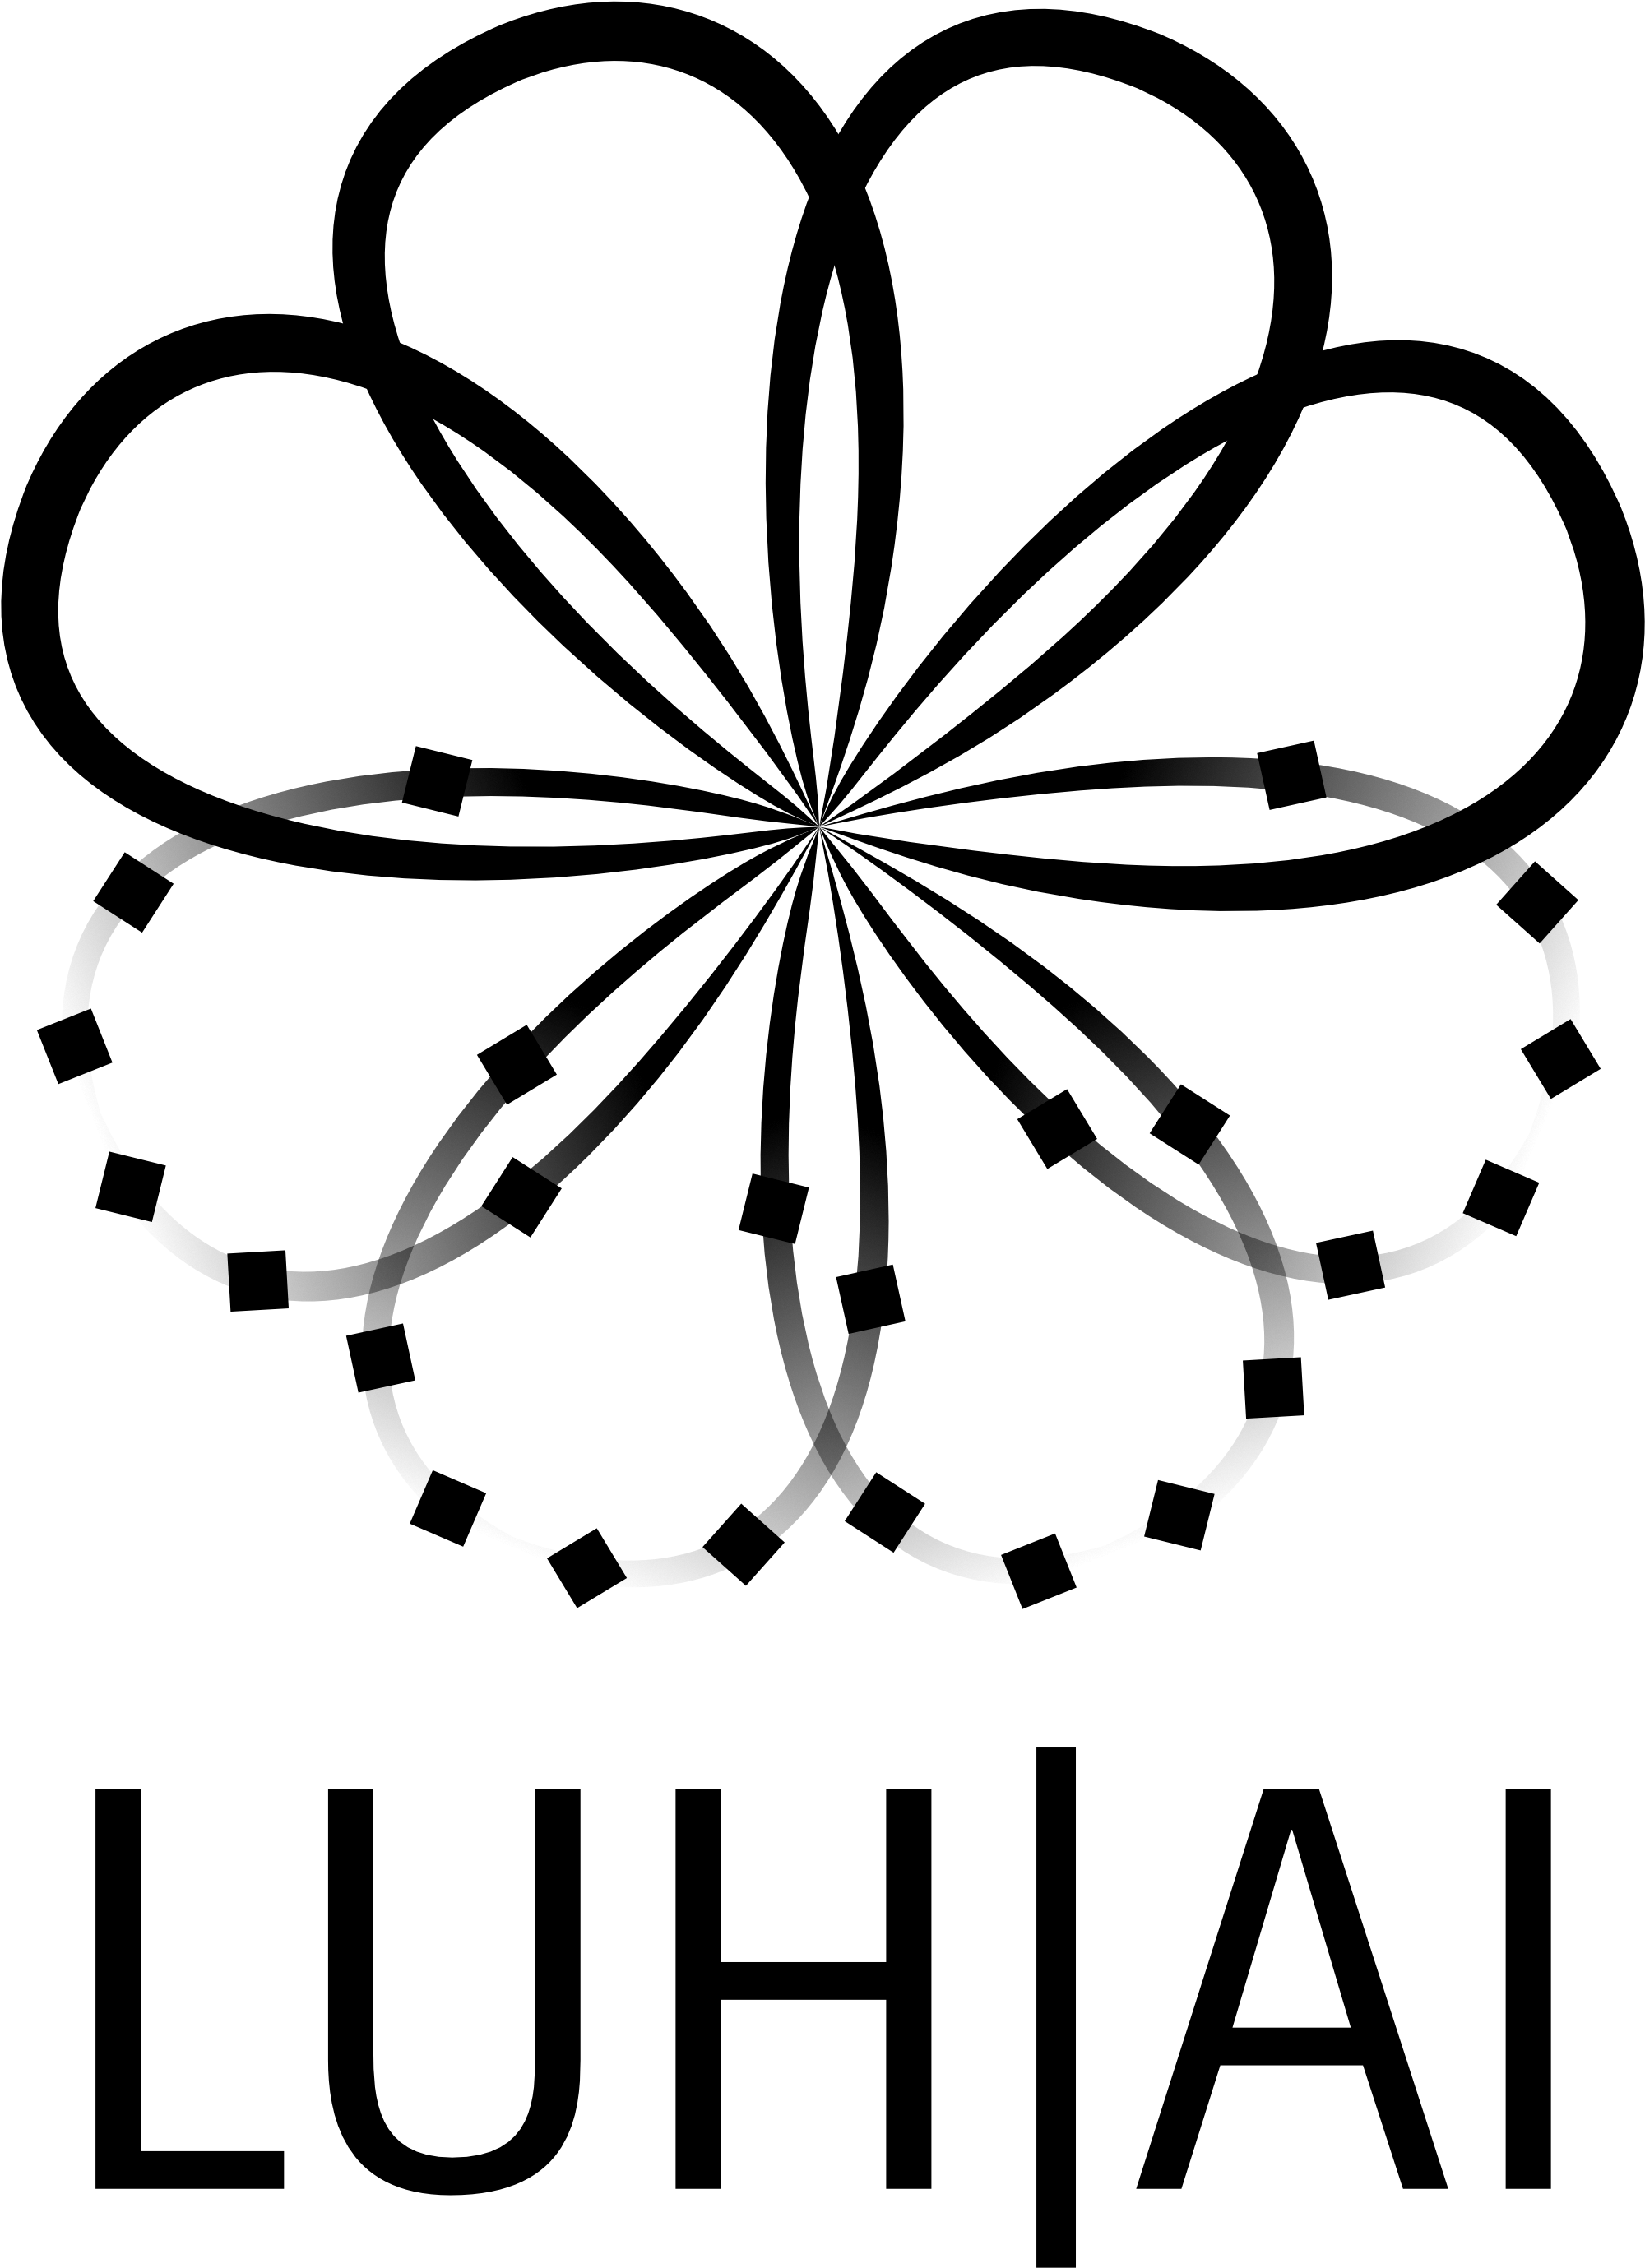
\includegraphics[height=\logoheight]{../latex_main/figures/logo_short_highres_black}\qquad

\includegraphics[height=\logoheight]{../latex_main/figures/Leibniz-AI-Academy_Logo}\qquad
%
\includegraphics[height=\logoheight]{../latex_main/figures/L3S.jpg}	
}
\date{\hspace{0.5em} {
\includegraphics[height=1.5em]{../latex_main/figures/Cc-by-nc-sa_icon.svg.png}}; extension of \href{https://ds100.org/fa21/}{[DS100]}
}


%%% Custom Packages
%----------------------------------------------------------------------
% Create dummy content
\usepackage{blindtext}

% Adds a frame with the current page layout. Just call \layout inside of a frame.
\usepackage{layout}


%%% Macros
%\renewcommand{\vec}[1]{\mathbf{#1}}
% \usepackage{bm}
%\let\vecb\bm

\title[Data Cleaning]{DS: Data Cleaning}
\subtitle{Motivation}

\graphicspath{ {./figure/} }
%\institute{}

\date{\hspace{0.5em}{
\includegraphics[height=1.5em]{../latex_main/figures/Cc-by-nc-sa_icon.svg.png}}; extension of DS100 and Ziawasch Abedjan}

\begin{document}
	
	\maketitle


% Slide 2
\begin{frame}[c]
    \frametitle{But, what do data scientists actually do?}

    \centering
    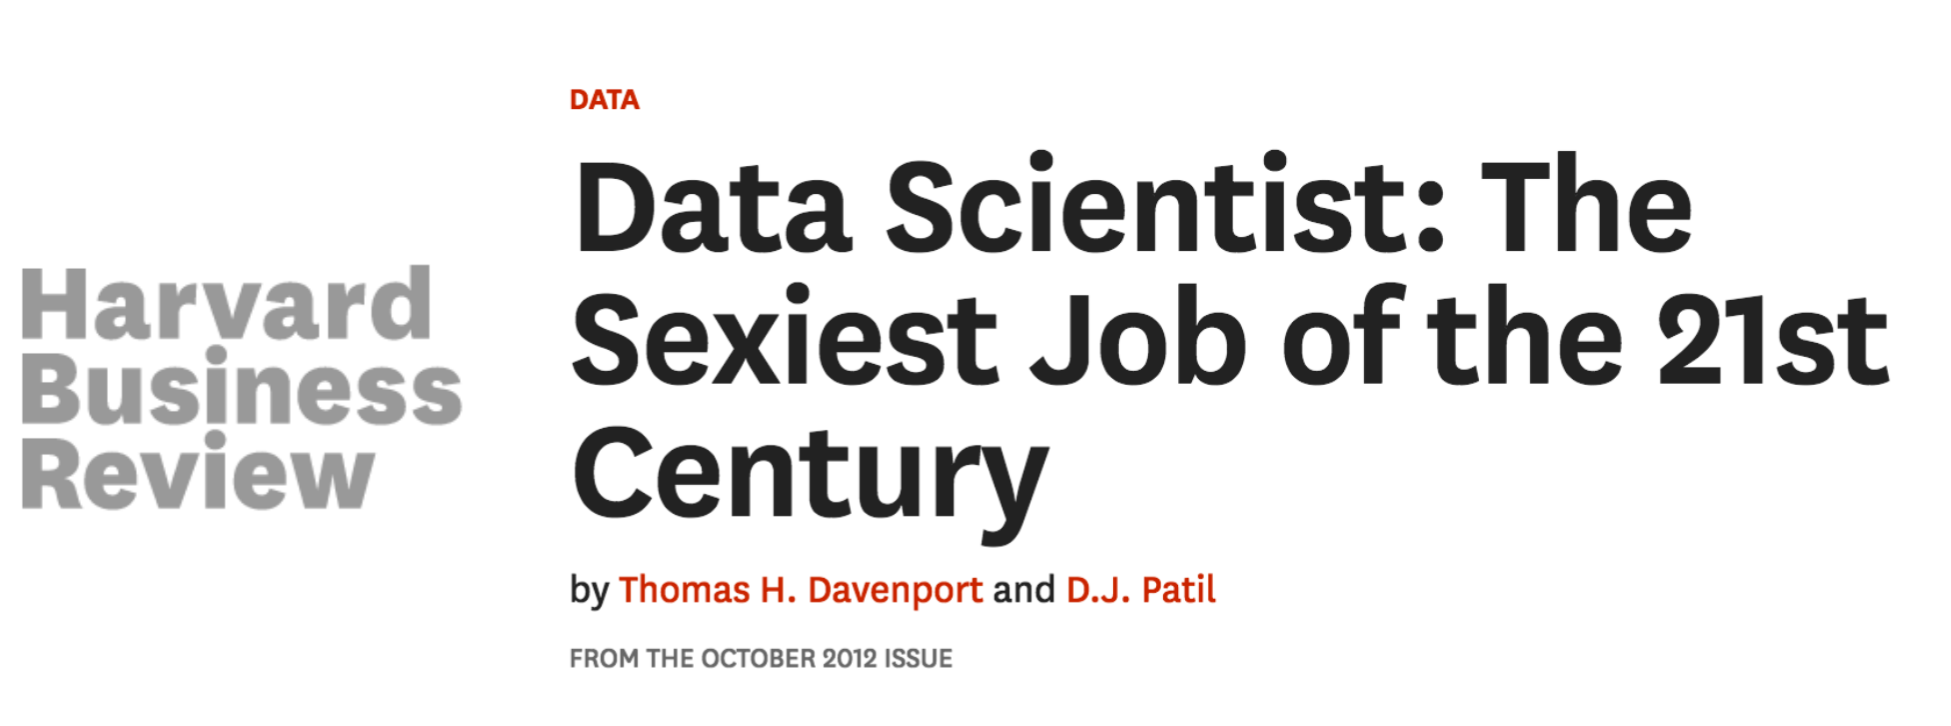
\includegraphics[width=1.0\textwidth]{bild1_harvard}
    
\end{frame}

% Slide 3 - Slide 4
\begin{frame}[c]
    \frametitle{CrowdFlower’s Data Science Report 2016}

     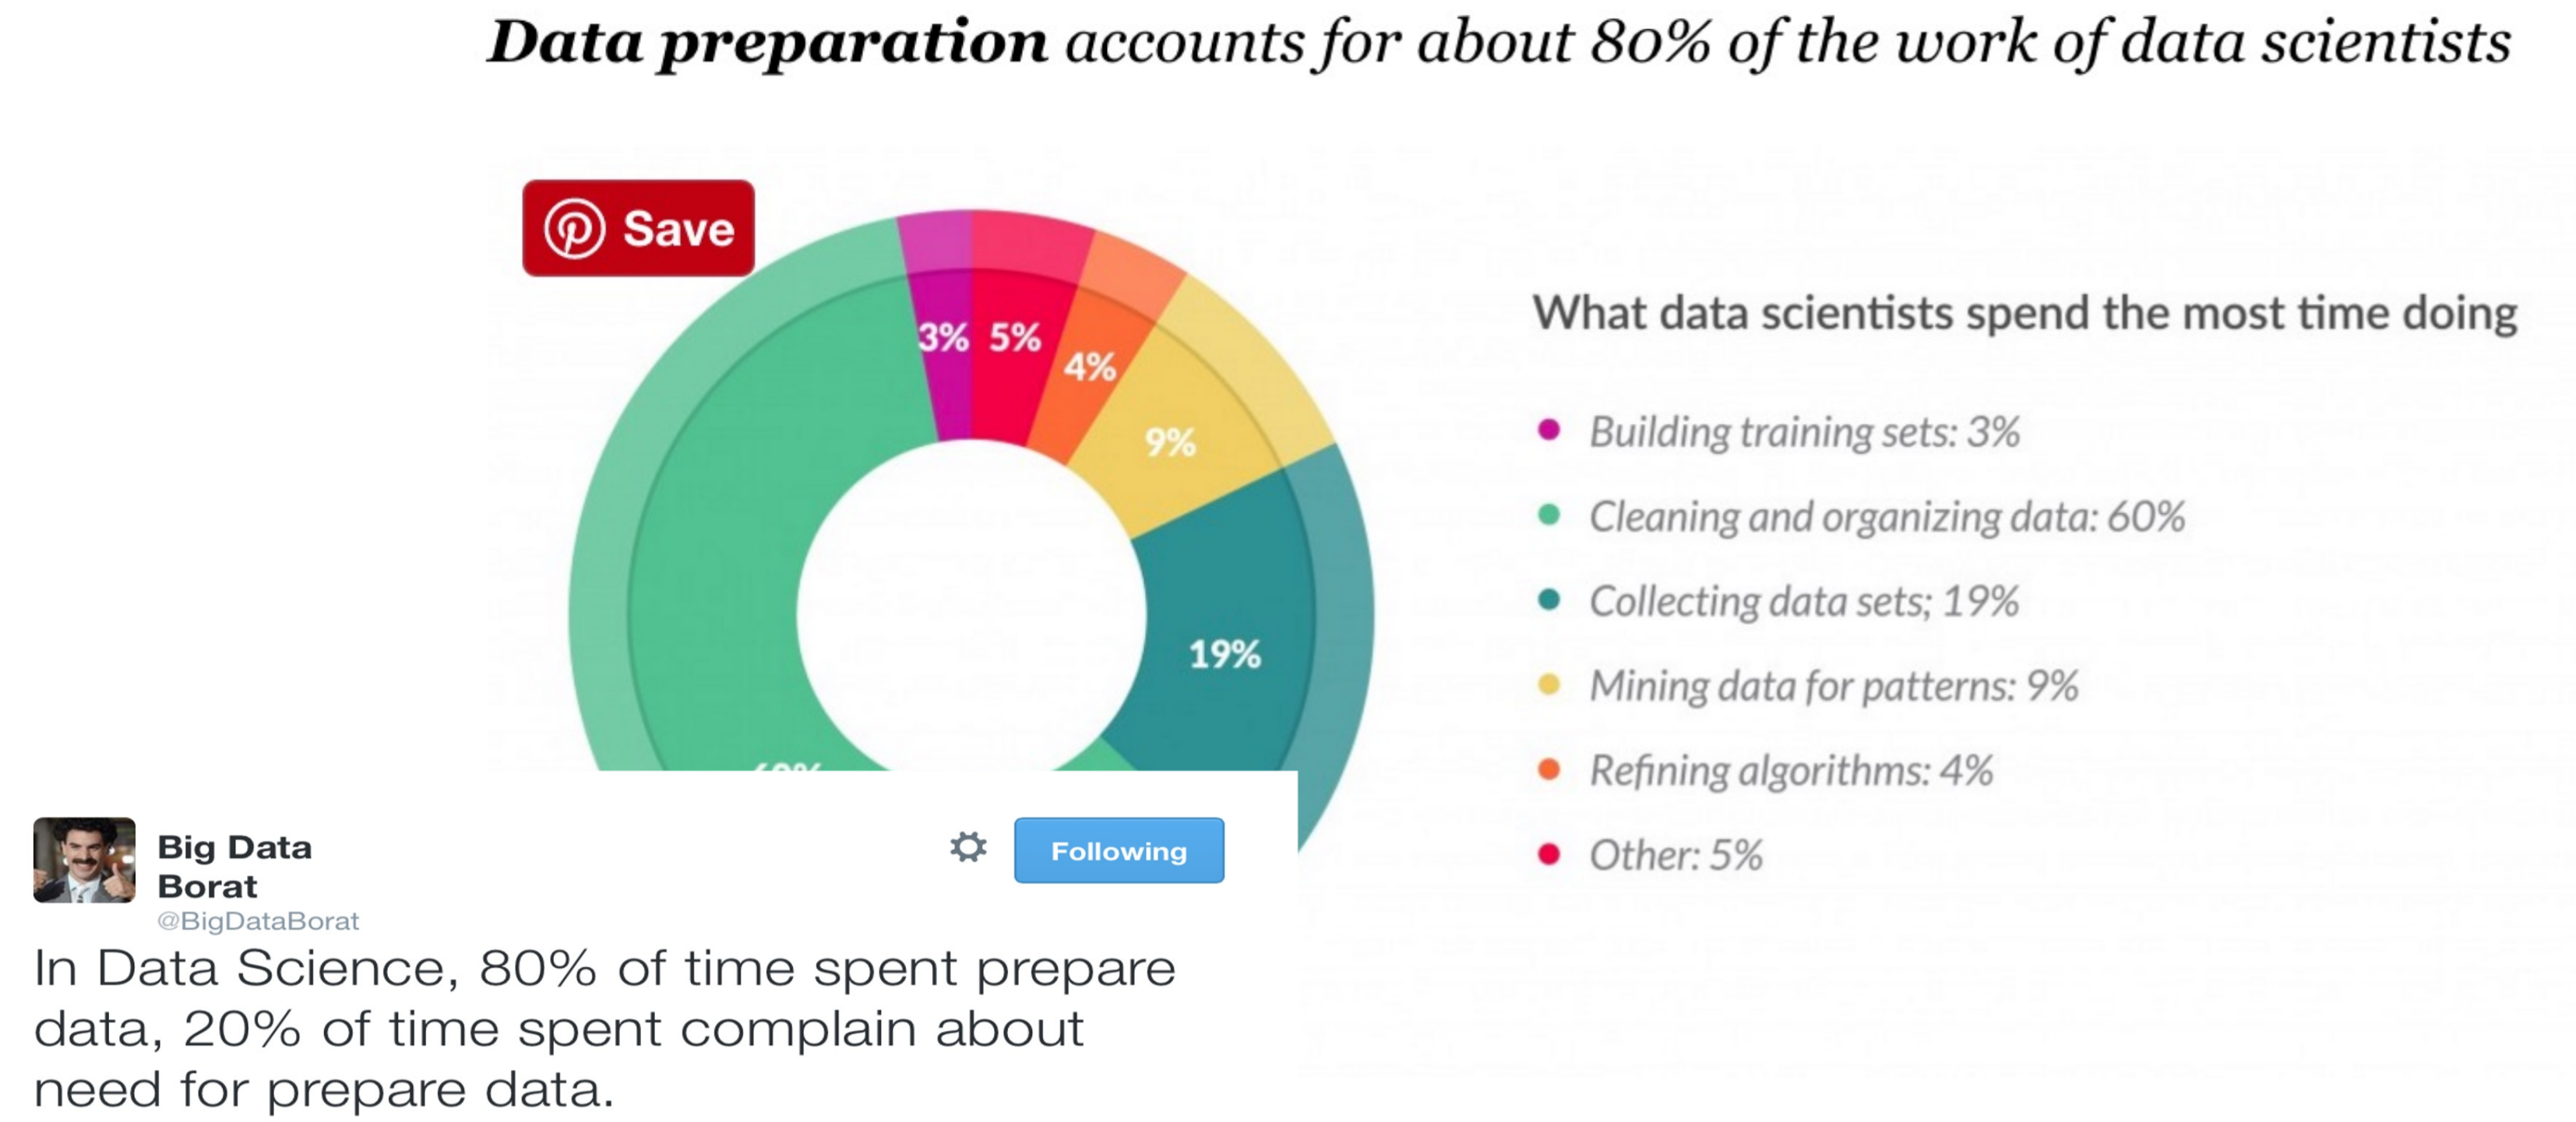
\includegraphics[width=1.0\textwidth]{bild2_data_prep}
    
\end{frame}

\begin{frame}[c]
    \frametitle{CrowdFlower’s Data Science Report 2016}

    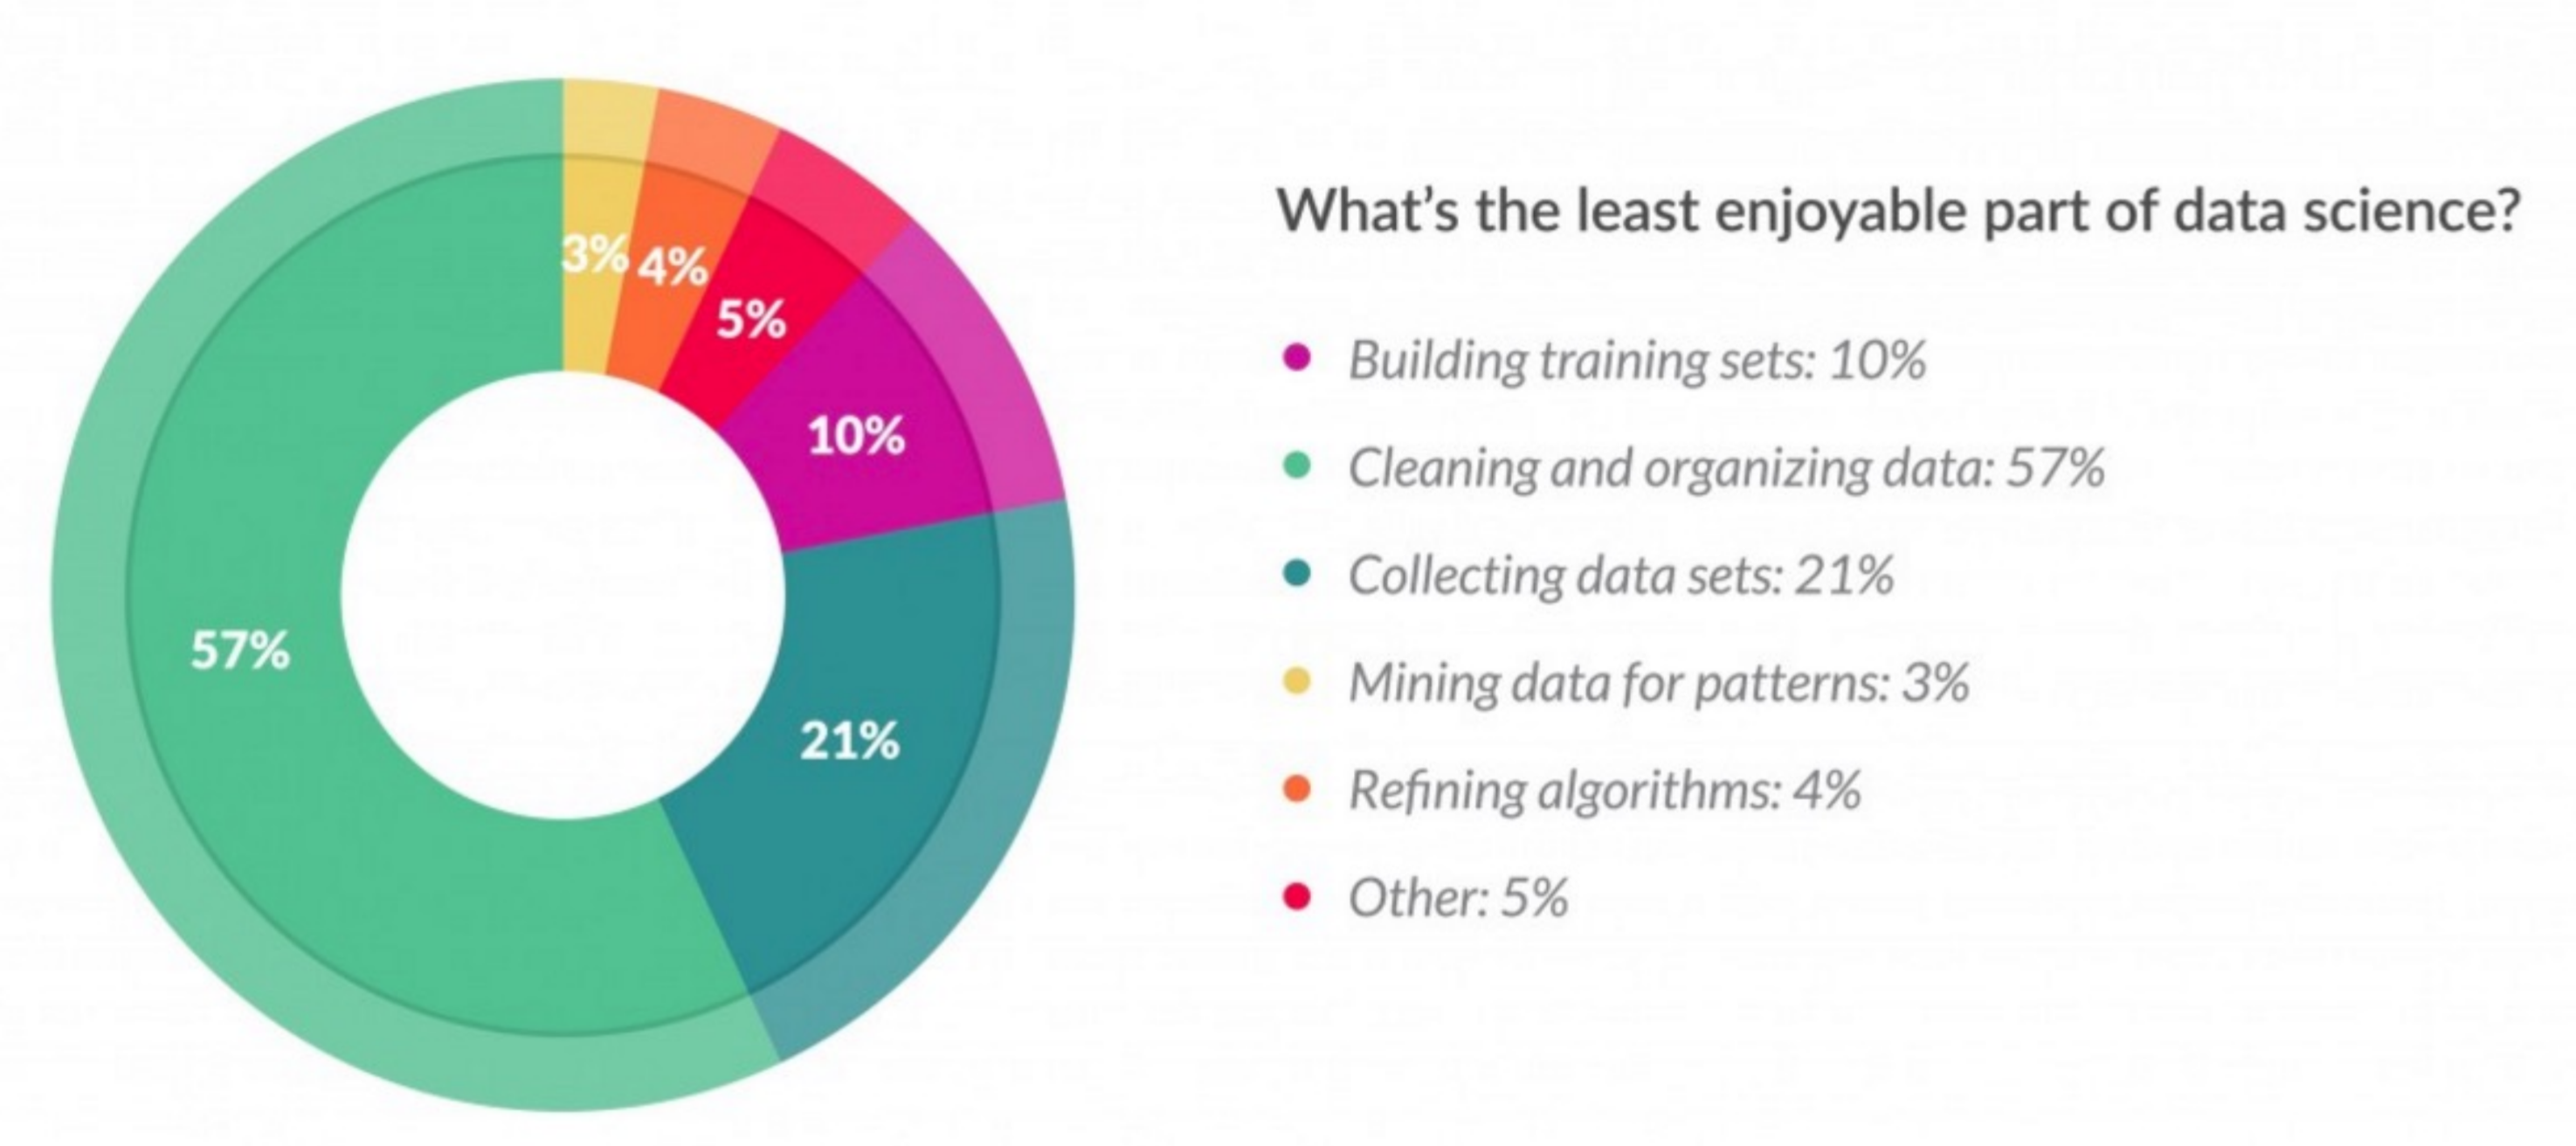
\includegraphics[width=1.0\textwidth]{bild3_least_enjoyable_thing}
\end{frame}

% Slide 5
\begin{frame}[c]{The 3rd V: Variety, the 800 pound Gorilla in the Corner}

    \centering
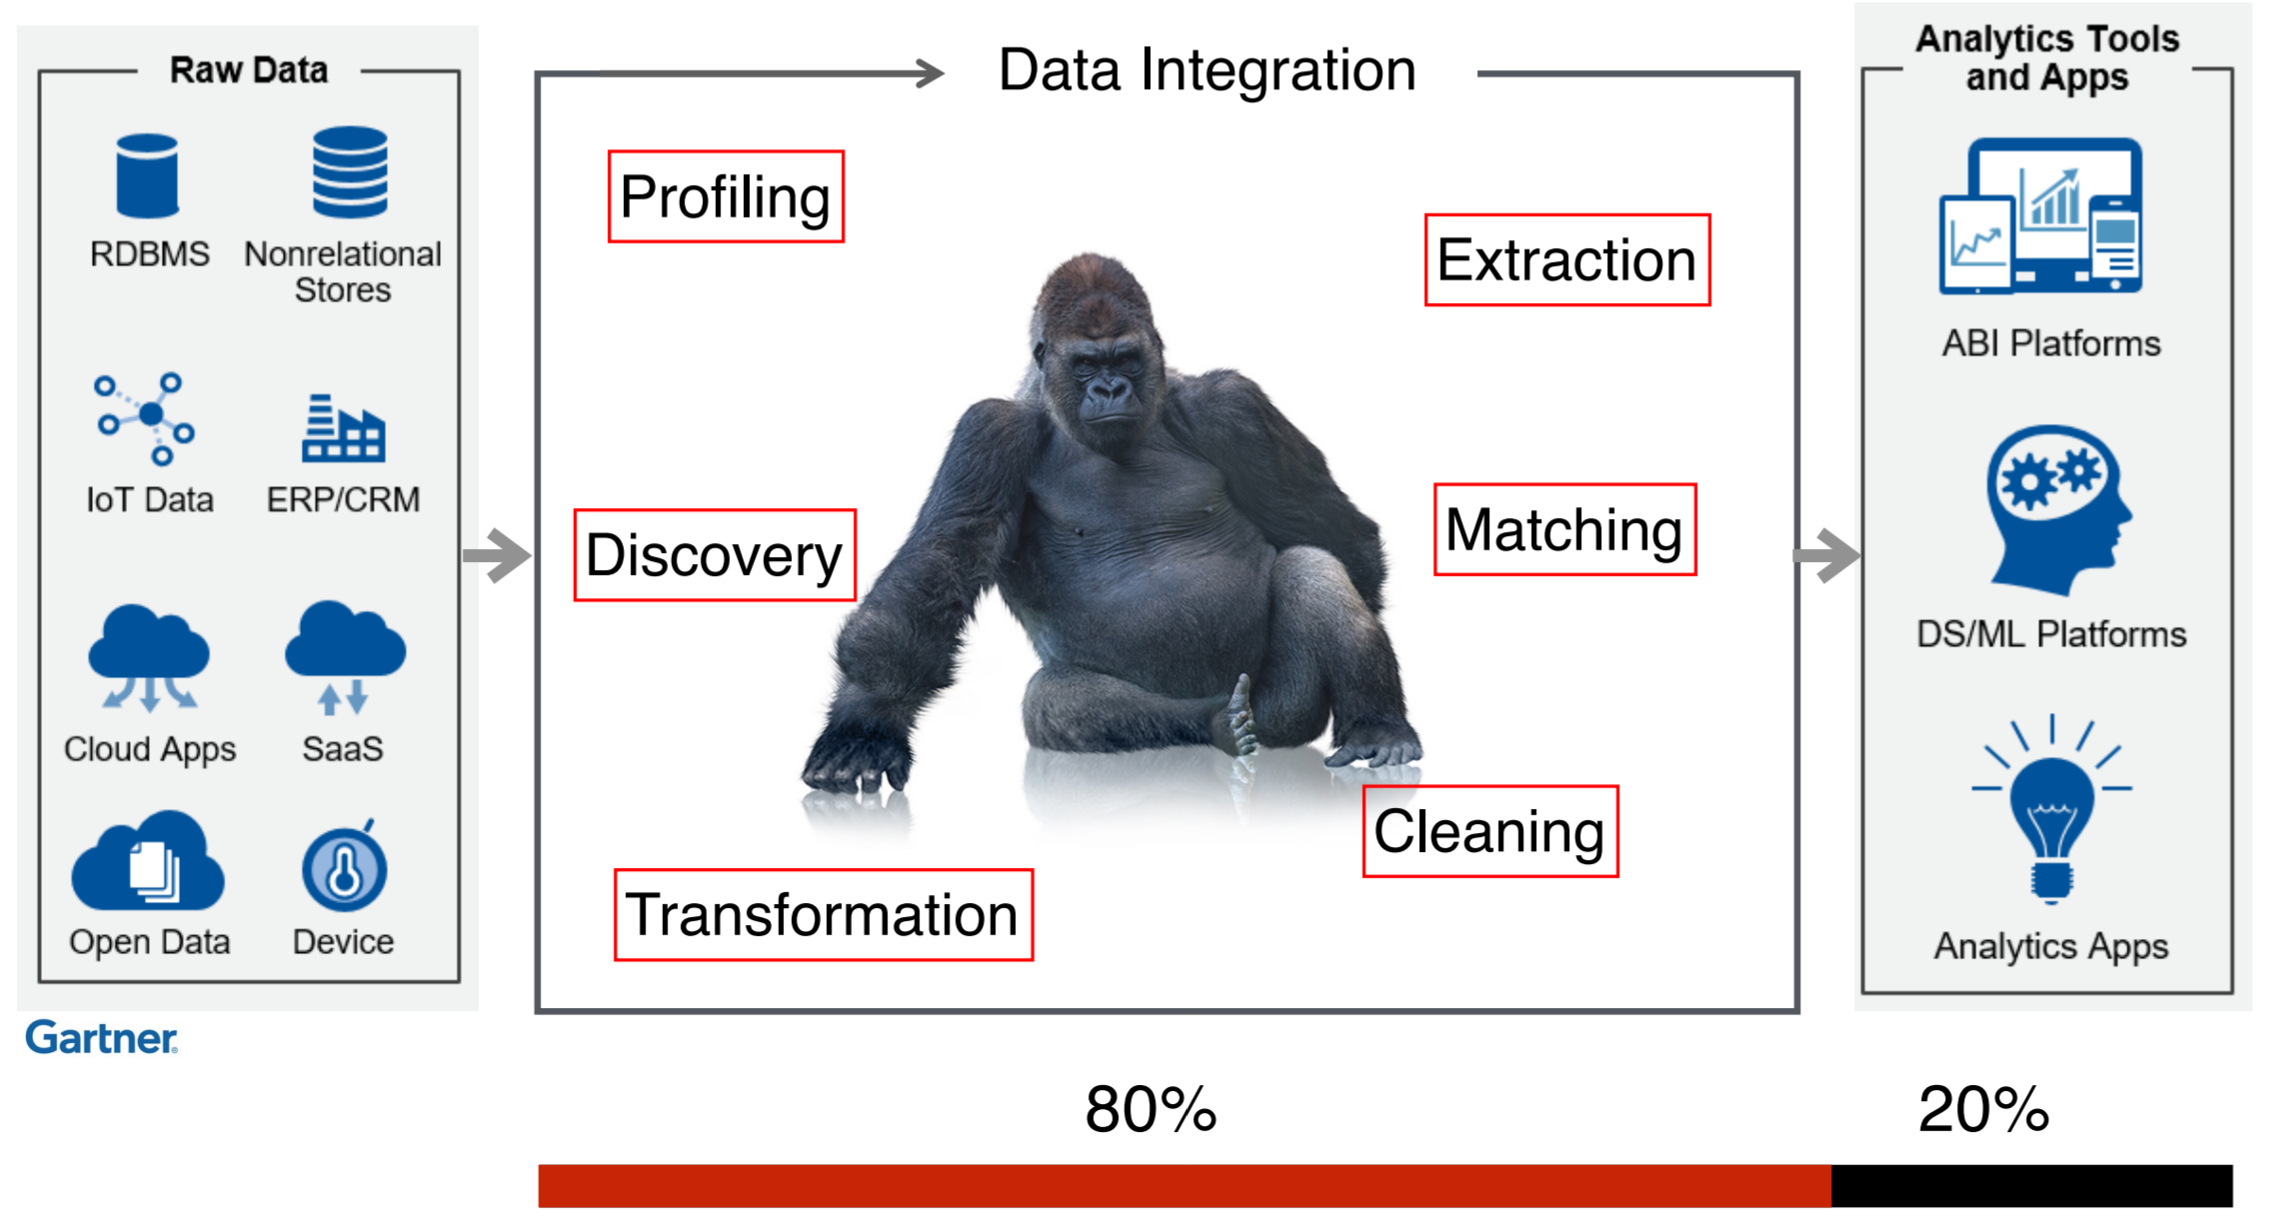
\includegraphics[width=1.0\textwidth]{bild4_gorilla}
    
     “Data Integration is the 800-pound Gorilla in the Corner, and everyone's got it in spades” - Michael Stonebraker, MIT
\end{frame}

% Slide 6
\begin{frame}[c]{Information Integration: An old problem}
    \begin{itemize}
        \item On the research agenda since 50 years.
        \item Early systems in the 1970s.
        \item Manual integration earlier
        \item New problems
        \begin{itemize}
            \item Many, many sources
            \item Heterogeneity
            \item New types of data (XML, GIS, etc.)
            \item New types of queries (search, UDFs,...)
            \item New types of results (ranking, visualization, ...) 
            \item New types of users (laymen, manager, admins, ...)
        \end{itemize}
    \end{itemize}
    \textit{Alon Halevy: “It’s plain hard!” (2004)}
\end{frame}

% Slide 7
\begin{frame}[c]{Why is it so difficult?}
    \begin{itemize}
        \item Systems reasons: 
        \begin{itemize}
            \item managing different platforms
            \item query processing
        \end{itemize}
        \item Social reasons:
        \begin{itemize}
            \item Locating and capturing relevant data in the enterprise
            \item Conciving people to share data fiefdoms
            \item Privacy and performance implications
        \end{itemize}
        \item Logic reasons: 
        \begin{itemize}
            \item Schema and data heterogeneity.
            \item Challenge independent of integration architecture!
        \end{itemize}
    \end{itemize}
\end{frame}

% Slide 8 - Data Preparation
\begin{frame}[c]{Data Preparation or Exploratory Data Analysis}

\textbf{``Getting to know the data''}

    \begin{itemize}
        \item Transform, visualize, summarize data to build understanding.
        \begin{itemize}
            \item Build/confirm understanding of the data and its provenance
            \item Identify and address potential issues in the data
            \item Inform the subsequent analysis 
            \item discover potential hypothesis … (be careful!)
        \end{itemize}
        \item EDA is open-ended analysis.
        \begin{itemize}
            \item Be willing to find something surprising
        \end{itemize}
    \end{itemize}
\end{frame}

% Slide 9 - Key Data Properties
\begin{frame}[c]{Key Data Properties to Consider in EDA}
    \begin{itemize}
        \item \textbf{Structure} -- the “shape” of a data file.
        \item \textbf{Granularity} -- how fine/coarse is each datum.
        \item \textbf{Scope} -- how (in)complete is the data.
        \item \textbf{Temporality} -- how is the data situated in time.
        \item \textbf{Faithfulness} --how well does the data capture “reality”.
    \end{itemize}
\end{frame}

	
\end{document}